% =====================================================================
%  附录 AR：电源与储能——从脉冲电源到电网接口（注明出处）
%  数值唯一来源：tools/calc/appAR_calc.py（只 print，输出 tools/calc/appAR_calc.txt）
%  单位口径：SI；功率写成 W/MW，能量写成 J/GJ，电压写成 V/kV
%  与其他附录的分工：附录 AM 管磁体与失超保护（本附录只接它的低温电耗），
%  附录 M 管加热与电流驱动（本附录只把它当负载），附录 V 管破裂的物理过程
%  （本附录只算缓解所需的脉冲功率），附录 Z 管电厂总体（本附录补电的支路）。
%  版权口径：只复算、不复制原书表格与图；直接引用处写「不复制」并标出处。
% =====================================================================
\section{电源与储能：电厂里的三本能量账}
\label{sec:app-ar-chain}

聚变电厂和一台实验装置最不一样的地方，不是等离子体，而是\emph{电}。实验装置从电网买电，只要把
等离子体点亮就算成功；电厂则要把电卖回去，于是每一瓦「自己用掉的电」都要从毛利里扣掉。这一节先把
账本摊开：一个聚变电厂的电，不是一笔账，而是三本。

第一本是\textbf{稳态账}——等离子体持续燃烧时，厂内始终有负荷在吃电：加热与电流驱动、低温制冷、
泵与加料、诊断与控制。这些负荷的总和叫\textbf{环流功率}（recirculating power）。第二本是
\textbf{脉冲账}——如果装置是脉冲运行的，每次放电都要把中心螺线管的电流从负拉到正，这笔能量在放电
开始前就得先存下来；同样的能量若在十秒内放出去，瞬时功率可以是稳态负荷的好几倍。第三本是
\textbf{瞬态账}——破裂缓解、快控线圈、失电保护，这些动作的能量不大，但要求在毫秒里把功率交出去。

先把稳态账算清楚。取 D1 工作点：聚变功率 $P_\mathrm{fus}=556.5$ MW，全部中子与 $\alpha$ 粒子的
能量都沉积进包层，于是热功率 $P_\mathrm{th}=5.565\times10^{8}$ W。设热电转换效率
$\eta_\mathrm{th}=0.40$，毛电功率

\begin{equation}
P_\mathrm{gross}=\eta_\mathrm{th}P_\mathrm{th}=0.40\times5.565\times10^{8}
=2.226\times10^{8}\ \mathrm{W}=222.6\ \mathrm{MW}.
\label{eq:app-ar-gross}
\end{equation}

厂内负荷按附录 M（加热与电流驱动）与附录 AM（磁体与低温）的口径取三项：电流驱动
$P_\mathrm{CD}=50.0$ MW、低温 $P_\mathrm{cryo}=13.4157$ MW（即附录 AM 的 $1.31333+12.1024$ MW）、
其余厂用电 $P_\mathrm{plant}=8.0$ MW。送到负载的电是

\begin{equation}
P_\mathrm{deliv}=P_\mathrm{CD}+P_\mathrm{cryo}+P_\mathrm{plant}
=50.0+13.4157+8.0=71.4157\ \mathrm{MW}.
\label{eq:app-ar-deliv}
\end{equation}

电源本身有损耗。设变换效率 $\eta_\mathrm{conv}=0.97$，则从发电机母线取走的电是

\begin{equation}
P_\mathrm{rec}=\frac{P_\mathrm{deliv}}{\eta_\mathrm{conv}}
=\frac{71.4157}{0.97}=73.6244\ \mathrm{MW},
\qquad
P_\mathrm{loss}=P_\mathrm{rec}-P_\mathrm{deliv}=2.20873\ \mathrm{MW}.
\label{eq:app-ar-recirc}
\end{equation}

净送出电与环流份额、电厂净效率定义为

\begin{equation}
\begin{aligned}
P_\mathrm{net}&=P_\mathrm{gross}-P_\mathrm{rec}=222.6-73.6244=148.976\ \mathrm{MW},\\
f_\mathrm{rec}&=\frac{P_\mathrm{rec}}{P_\mathrm{gross}}=33.0748\%,
\qquad
\eta_\mathrm{net}=\frac{P_\mathrm{net}}{P_\mathrm{th}}=26.7701\%.
\end{aligned}
\label{eq:app-ar-net}
\end{equation}

注意 $\eta_\mathrm{net}$ 比 $\eta_\mathrm{th}$ 低了十三个百分点：热电转换定了 40\% 的上限，
而环流功率又从里面拿走了三成三。换个说法，每送出 1 MW 净电，背后要有
$P_\mathrm{th}/P_\mathrm{net}=3.73551$ MW 的聚变功率在烧。

再看脉冲账。中心螺线管的电感取 $L_\mathrm{CS}=10$ H，电流摆幅 $\pm40$ kA，则磁储能

\begin{equation}
E_\mathrm{CS}=\tfrac12 L_\mathrm{CS}I_\mathrm{pk}^2
=\tfrac12\times10\times(4.0\times10^{4})^2=8.0\times10^{9}\ \mathrm{J}=8\ \mathrm{GJ}.
\label{eq:app-ar-cs}
\end{equation}

这笔能量要在爬升阶段交出去。若爬升用 $\Delta t=10$ s，平均功率

\begin{equation}
\begin{aligned}
P_\mathrm{ramp}&=\frac{E_\mathrm{CS}}{\Delta t}=\frac{8.0\times10^{9}}{10}
=8.0\times10^{8}\ \mathrm{W}=800\ \mathrm{MW},\\
\frac{\mathrm{d}I}{\mathrm{d}t}&=\frac{2I_\mathrm{pk}}{\Delta t}=8000\ \mathrm{A/s},
\qquad
V_\mathrm{CS}=L_\mathrm{CS}\frac{\mathrm{d}I}{\mathrm{d}t}=80\ \mathrm{kV}.
\end{aligned}
\label{eq:app-ar-ramp}
\end{equation}

$800$ MW 是净电 $148.976$ MW 的 $5.37001$ 倍——单靠厂内发电机供不起，所以脉冲装置要么把爬升拉长
（$\Delta t=100$ s 时平均功率降到 $80$ MW），要么在厂内放一组储能把这些能量先攒起来。
这就是第三本账旁边的那个「水库」。

最后是瞬态账。破裂缓解要在 $10$ ms 里交出 $E_\mathrm{mit}=2.0$ MJ，平均功率
$E_\mathrm{mit}/\Delta t_\mathrm{mit}=2.0\times10^{8}$ W $=200$ MW，是稳态环流功率的
$2.71649$ 倍；单看能量它只有环流功率运行 $27.1649$ ms 的量，值钱的是\emph{时间}。

\begin{table}[htbp]
\centering
\small
\caption{电厂的三本能量账：稳态、脉冲、瞬态}
\label{tab:app-ar-books}
\begin{tabular}{p{2.6cm}p{3.5cm}p{3.3cm}p{3.6cm}}
\hline
账本 & 代表量 & 数值 & 对设计的要求 \\
\hline
稳态 & 毛电 $P_\mathrm{gross}$ & $222.6$ MW & 热电转换效率定上限 \\
稳态 & 环流 $P_\mathrm{rec}$ & $73.6244$ MW（$33.0748\%$） & 每一项负荷都要单独省 \\
脉冲 & 螺线管储能 $E_\mathrm{CS}$ & $8$ GJ & 要么拉长爬升，要么上储能 \\
脉冲 & 10 s 爬升功率 & $800$ MW（净电的 $5.37001$ 倍） & 电网瞬时能力或厂内储能 \\
瞬态 & 破裂缓解脉冲 & $200$ MW / $10$ ms & 毫秒级开关与能量 \\
瞬态 & 等效环流时间 & $27.1649$ ms & 能量小、时间贵 \\
\hline
\end{tabular}
\end{table}

\begin{tip}{三本账要分开算}{tip-app-ar-books}
把爬升功率、稳态环流和瞬态脉冲加成一个「总电源容量」，是这类设计里最常见的错。三者的时间尺度
相差四个数量级，能提供的设备也完全不同：稳态靠电网与发电机，脉冲靠储能与飞轮，瞬态靠电容与快
开关。混在一起算，结果一定偏大，然后被「成本太高」这个结论误导。
\end{tip}


\textbf{出处：}电厂能量账与再循环功率的口径见 Freidberg, \emph{Plasma Physics and Fusion Energy}
（2007）第 5 章；磁体与低温电耗取本书附录 AM 的同一组数值；中心螺线管的电流摆幅与爬升时间取量级
口径，用于说明「脉冲账」的量级关系。本附录不复印原书图表。

\section{变流器与纹波：十二脉波为什么是标准}
\label{sec:app-ar-converter}

线圈电源不是电池，它把电网的交流变成几十千安的可控直流。这个变换留下两个副产品：\textbf{纹波}
与\textbf{谐波}。

把三相桥式整流的六个臂按一定相位拼起来，就得到\textbf{脉波数}。脉波数越多，整流后的电压越平：
六脉波的纹波系数约 $13.4\%$，十二脉波约 $4.2\%$，二十四脉波约 $2.1\%$——十二脉波是工程折中的
标准选择，纹波只有六脉波的 $1/3.19048$。理想空载直流电压记作 $U_\mathrm{d0}$，带触发角
$\alpha$ 时

\begin{equation}
U_\mathrm{d}=U_\mathrm{d0}\cos\alpha .
\label{eq:app-ar-ud}
\end{equation}

取 $U_\mathrm{d0}=24$ kV、$\alpha=15^\circ$，则 $U_\mathrm{d}=23.1822$ kV，$\cos\alpha=0.965926$。
若直流侧要送 $I_\mathrm{d}=40$ kA，则直流功率

\begin{equation}
P_\mathrm{d}=U_\mathrm{d}I_\mathrm{d}=2.31822\times10^{4}\times4.0\times10^{4}
=9.27289\times10^{8}\ \mathrm{W}=927.289\ \mathrm{MW},
\label{eq:app-ar-pd}
\end{equation}

对应交流侧视在功率约 $986.8$ MVA。请留意这是\emph{峰值工况}：线圈电源按峰值设计，按平均值运行。

脉波数还决定谐波。$p$ 脉波的交流侧电流只含 $kp\pm1$ 次谐波，相对幅值近似 $1/n$：

\begin{equation}
n=kp\pm1,\qquad \frac{I_n}{I_1}\approx\frac{1}{n}.
\label{eq:app-ar-harm}
\end{equation}

十二脉波的最低次是 11 次与 13 次，相对幅值 $0.0909091$ 与 $0.0769231$，两者合成 $0.167832$；
六脉波则会多出 5 次（$0.2$）与 7 次（$0.142857$），这正是十二脉波被当成标准的原因。
谐波要在并网点滤掉，滤波器按下式调谐：

\begin{equation}
\omega_n=\frac{1}{\sqrt{L_\mathrm{f}C_\mathrm{f}}},\qquad
L_\mathrm{f}=\frac{1}{(2\pi n f_0)^2C_\mathrm{f}} .
\label{eq:app-ar-filter}
\end{equation}

取 $C_\mathrm{f}=100\ \mu$F、$f_0=50$ Hz，11 次谐波要 $0.837365$ mH，13 次要 $0.599534$ mH。

最后是无功。相控整流在触发角 $\alpha$ 下要从电网吸收无功：

\begin{equation}
Q\approx P\tan\alpha .
\label{eq:app-ar-q}
\end{equation}

按毛电 $222.6$ MW 与 $\alpha=15^\circ$（$\tan\alpha=0.267949$）估，$Q=59.6455$ MVAr。
换相角 $\mu$ 会让功率因数再降一点：$\cos(\alpha+\mu/2)=0.939693$，比 $\cos\alpha$ 低
$2.71586\%$。

\begin{table}[htbp]
\centering
\small
\caption{脉波数与纹波、谐波的关系（纹波系数为文献级典型值）}
\label{tab:app-ar-pulse}
\begin{tabular}{p{1.9cm}p{2.3cm}p{2.7cm}p{3.0cm}p{3.1cm}}
\hline
脉波数 & 纹波系数 & 最低谐波次数 & 相对幅值 & 典型用途 \\
\hline
6 & $13.4\%$ & 5、7 & $0.2$、$0.142857$ & 小功率线圈电源 \\
12 & $4.2\%$ & 11、13 & $0.0909091$、$0.0769231$ & 大电流线圈电源标准 \\
24 & $2.1\%$ & 23、25 & 更小 & 对纹波极敏感场合 \\
\hline
\end{tabular}
\end{table}

\begin{tip}{纹波不是噪声，是换相留下的缺口}{tip-app-ar-ripple}
纹波的频率是脉波数乘工频，不是随机噪声，因此它可以用滤波器算准、也可以在设计上避开。真正难对付
的是换相瞬间的电压缺口与由此产生的谐波电流，它们会直接落到并网点上，成为电网考核的指标。
\end{tip}


\textbf{出处：}脉波数、纹波系数与谐波次数的关系是电力电子教科书的标准内容，见 Rashid,
\emph{Power Electronics Handbook}（第 4 版）整流器一章与 Mohan、Undeland、Robbins,
\emph{Power Electronics}（第 3 版）第 5 章；触发角与换相角对功率因数的影响同源。本附录只取公式
与量级，不复印原书图表。
\begin{figure}[htbp]
\centering
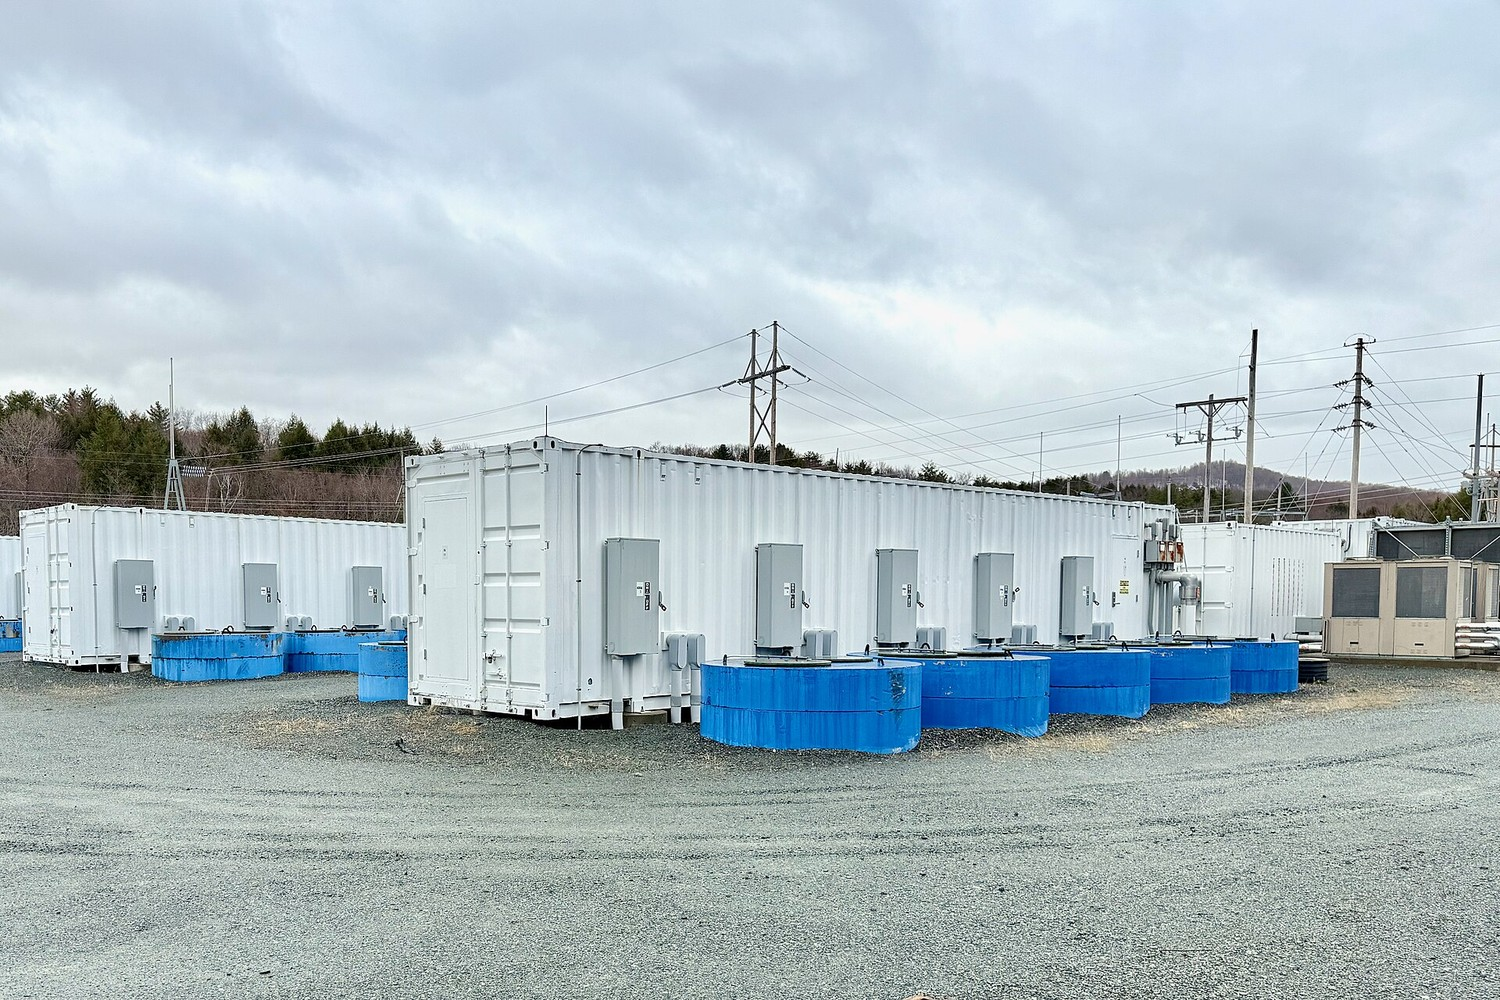
\includegraphics[width=0.78\textwidth]{../figures/flywheel_20mw.jpg}
\caption{把能量存在转子里：20 MW 飞轮储能。飞轮的能量是 $\frac12 I\omega^2$，能撑多久由功率与容量共同决定。这座电站的 200 台飞轮并机运行，正对应本章「储能：飞轮、电容与它们能撑多久」那笔账。}
\label{fig:photo-appar2}
\figsource{Z22，CC BY-SA 4.0（Wikimedia Commons），链接见 figures/CREDITS.md。}
\end{figure}

\section{储能：飞轮、电容与它们能撑多久}
\label{sec:app-ar-storage}

脉冲账里的 8 GJ 不可能靠电网瞬时给。厂内储能有三条路：把能量存在\textbf{转动惯量}里（飞轮）、
存在\textbf{电场}里（电容）、存在\textbf{磁场}里（电感），或者干脆买电池。四条路的物理上限各不
相同，选哪条由「要撑多久」和「要多快」共同决定。

飞轮的能量是转动动能：

\begin{equation}
E=\tfrac12 I\omega^2 .
\label{eq:app-ar-flywheel}
\end{equation}

取实心圆盘 $m=20000$ kg、$r=2.0$ m，则 $I=\tfrac12mr^2=40000\ \mathrm{kg\,m^2}$；转速
$3000$ rpm 对应 $\omega=314.159$ rad/s，储能

\begin{equation}
E=\tfrac12\times4.0\times10^{4}\times(314.159)^2=1.97392\times10^{9}\ \mathrm{J}=1.97392\ \mathrm{GJ}.
\label{eq:app-ar-flywheel2}
\end{equation}

但飞轮真正的限制不在轴承，而在\textbf{材料强度}。轮缘的环向应力随线速度平方增长：

\begin{equation}
\sigma=\rho v^2,\qquad v_\mathrm{max}=\sqrt{\sigma/\rho}.
\label{eq:app-ar-vmax}
\end{equation}

$3000$ rpm 时边缘线速度 $v=\omega r=628.319$ m/s，钢（$\rho=7850\ \mathrm{kg/m^3}$）的应力
$\rho v^2=3.09906\times10^{9}$ Pa $=3.09906$ GPa，已经超过钢的强度 $1.0$ GPa——
这只钢飞轮会散架。钢允许的线速度只有 $v_\mathrm{max}=356.915$ m/s（对应 $1704.15$ rpm）；
换碳纤维（$\rho=1600\ \mathrm{kg/m^3}$、$\sigma=3.0$ GPa）允许 $1369.31$ m/s，是钢的
$3.8365$ 倍，同样质量与半径下能存 $9.375$ GJ。

电容的能量存在电场里：

\begin{equation}
E=\tfrac12CV^2,\qquad C=\frac{2E}{V^2}.
\label{eq:app-ar-cap}
\end{equation}

存 $2.0$ MJ 而电压取 $20$ kV，需要 $C=0.01$ F $=10$ mF；若手里只有 $5$ mF，则要把电压升到
$28.2843$ kV。这笔能量在 $10$ ms 内放出去就是 $200$ MW，平均电流 $10$ kA、峰值电流 $20$ kA——
这正是破裂缓解要的「快而短」。

电感储能是磁体的副产品：

\begin{equation}
E=\tfrac12LI^2 .
\label{eq:app-ar-ind}
\end{equation}

附录 AM 的螺线管口径（$L=10$ H、$I=40$ kA）给出 $8$ GJ，与脉冲账完全对上。它的麻烦在保护：
$\mathrm{d}I/\mathrm{d}t$ 不能突然切断，否则电压会失控；$R=1$ m$\Omega$ 的泄能回路时间常数
$L/R=10000$ s，是「慢放」而不是「快放」的器件。

放电能撑多久，是能量除以功率：

\begin{equation}
\Delta t_\mathrm{dis}=\frac{E}{P}.
\label{eq:app-ar-discharge}
\end{equation}

$1.97392$ GJ 的飞轮按 $100$ MW 放电能撑 $19.7392$ s；同样 $8$ GJ 可以撑 $80$ s。作为对照，
厂用电 $8$ MW 撑一小时需要 $28.8$ GJ，$1$ MWh 折合 $3.6\times10^{9}$ J——飞轮只相当于
$0.548311$ MWh 的电池，却能在几十毫秒里把功率交出去。储能选型的本质，是在\emph{能量密度}与
\emph{功率密度}之间挑一个点。

\begin{table}[htbp]
\centering
\small
\caption{四条储能路线的物理上限（口径见正文）}
\label{tab:app-ar-storage}
\begin{tabular}{p{1.9cm}p{2.4cm}p{2.6cm}p{2.6cm}p{3.4cm}}
\hline
路线 & 能量公式 & 本附录例子 & 能撑多久 & 主要限制 \\
\hline
飞轮 & $\tfrac12I\omega^2$ & $1.97392$ GJ（$20000$ kg、$2.0$ m、$3000$ rpm） & $19.7392$ s（$100$ MW） & 材料强度 $\sigma=\rho v^2$ \\
电容 & $\tfrac12CV^2$ & $2.0$ MJ（$10$ mF、$20$ kV） & $10$ ms（$200$ MW） & 能量密度低（$40$ MJ/m$^3$） \\
电感 & $\tfrac12LI^2$ & $8$ GJ（$10$ H、$40$ kA） & 放电受保护限制 & 断路与电压失控 \\
电池 & 化学能 & $1$ MWh $=3.6\times10^{9}$ J & 小时级 & 功率密度与循环寿命 \\
\hline
\end{tabular}
\end{table}

\begin{tip}{飞轮的极限不是轴承，是材料强度}{tip-app-ar-flywheel}
「转速越高储能越多」只在材料撑得住时成立。$\sigma=\rho v^2$ 说明应力只跟线速度有关，与半径无关，
所以放大飞轮要放大半径而不是提高转速；碳纤维比钢强三倍多，正是因为它把 $v_\mathrm{max}$ 抬高了
$3.8365$ 倍——而能量按 $v^2$ 涨，于是同样的质量能存九倍多的能量。
\end{tip}


\textbf{出处：}飞轮的应力限制与比能量推导见 Genta, \emph{Kinetic Energy Storage}（1985）与
Bolund 等，\emph{Energy Conversion and Management} 48 (2007) 讨论飞轮储能的综述；电容与电感储能
的公式属电磁学基本内容；四条路线的对比口径参考 Dolan（编），\emph{Magnetic Fusion Technology}
（2013）储能与电源章。本附录不复制原书数值表。

\section{环流功率：电厂净效率的分母}
\label{sec:app-ar-recirculating}

环流功率 $73.6244$ MW 不是一个数，而是一张清单。按前面的口径拆开：电流驱动
$67.9122\%$、低温 $18.2218\%$、其他厂用电 $10.866\%$、变换损耗 $3\%$。要省电，只能从这张
清单上逐项省。

电流驱动是大头，这一项直接由等离子体的物理决定：同样的电流剖面与自举电流份额，需要的驱动功率
由附录 M 给出；本附录把它当负载，但要知道\textbf{科学增益}与\textbf{工程增益}是两件事：

\begin{equation}
Q_\mathrm{pl}=\frac{P_\mathrm{fus}}{P_\mathrm{CD}}=11.13,
\qquad
Q_\mathrm{eng}=\frac{P_\mathrm{net}}{P_\mathrm{rec}}=2.02345 .
\label{eq:app-ar-qeng}
\end{equation}

等离子体的科学增益可以是十几，但厂里的工程增益只有二点零——因为科学增益的分母只是驱动功率，
而工程增益的分母要把电网侧的全部损耗算进来。这也是为什么「点火」不是终点：点火只让 $P_\mathrm{CD}$
趋近于零，低温与厂用电还在。

灵敏度可以定量看。若电流驱动的电效率提高 $10\%$（省下 $5$ MW 的送出电），电厂净效率

\begin{equation}
\Delta\eta_\mathrm{net}=\frac{5.0}{556.5}=0.898473\ \text{个百分点},
\label{eq:app-ar-sens}
\end{equation}

即从 $26.7701\%$ 升到约 $27.67\%$。反过来，若想把环流份额压到 $25\%$，环流功率要降到
$55.65$ MW，相当于再削减 $17.9744$ MW——这比省下一项 $8$ MW 的厂用电还多一倍。

\begin{table}[htbp]
\centering
\small
\caption{稳态环流功率的分解与占比}
\label{tab:app-ar-recirc}
\begin{tabular}{p{3.0cm}p{2.4cm}p{2.2cm}p{5.3cm}}
\hline
项目 & 功率 & 占环流 & 说明 \\
\hline
加热与电流驱动 & $50.0$ MW & $67.9122\%$ & 由等离子体物理决定，最值得优化 \\
低温制冷 & $13.4157$ MW & $18.2218\%$ & 与附录 AM 同一口径 \\
其他厂用电 & $8.0$ MW & $10.866\%$ & 泵、加料、诊断、控制 \\
变换损耗 & $2.20873$ MW & $3\%$ & 电源效率 $0.97$ 的代价 \\
\hline
合计 & $73.6244$ MW & $100\%$ & 占毛电 $33.0748\%$ \\
\hline
\end{tabular}
\end{table}

\begin{tip}{环流功率是分母，不是余数}{tip-app-ar-recirc}
初学者常把环流功率当成「次要损失」，先算聚变再随便扣一点。它其实是分母：净电 $=P_\mathrm{gross}
-P_\mathrm{rec}$，两项都在百分之几十的量级，误差会直接放大到电价上。设计顺序上也一样——先问
「厂内要吃掉多少电」，再谈聚变功率要多大。
\end{tip}


\textbf{出处：}再循环功率与工程增益的定义见 Freidberg, \emph{Plasma Physics and Fusion Energy}
（2007）第 5 章与 Stacey, \emph{Fusion: An Introduction to the Physics and Technology of Magnetic
Confinement Fusion}（第 2 版，2011）电厂章；电流驱动功率的物理见本书附录 M 与 Wesson,
\emph{Tokamaks}（第 3 版，2004）电流驱动章。本附录不复制原书表格。

\section{电网接口：并网、频率响应与无功}
\label{sec:app-ar-grid}

电厂接的不是理想电压源，而是一张有惯性的网。电网的频率由所有同步机的转动惯量撑着，功率缺额会让
频率按

\begin{equation}
\frac{\mathrm{d}f}{\mathrm{d}t}=\frac{\Delta P}{2HS_\mathrm{grid}}
\label{eq:app-ar-rocof}
\end{equation}

下滑。取惯性常数 $H=5$ s、短路容量 $S_\mathrm{grid}=1000$ MVA、扰动 $\Delta P=100$ MW，则
变化率 $0.01$ Hz/s；若允许频率掉 $0.2$ Hz，留给保护与储能的时间是 $20$ s。

聚变厂的并网有几处特殊：一是厂用电占比不小——环流功率 $71.4157$ MW 相当于短路容量的
$7.14157\%$，净送出 $148.976$ MW 占 $14.8976\%$；二是电源整流会吸无功，$\alpha=15^\circ$ 时
$Q=59.6455$ MVAr，需要就地补偿把功率因数拉回 $0.965926$；三是黑启动。厂用电 $8$ MW 撑一小时需要

\begin{equation}
E_\mathrm{black}=P_\mathrm{plant}t=8.0\times10^{6}\times3600=2.88\times10^{10}\ \mathrm{J}=28.8\ \mathrm{GJ},
\label{eq:app-ar-black}
\end{equation}

比脉冲账的 $8$ GJ 还大——一台停下来的电厂，第一件难事是把自己点亮。

\begin{table}[htbp]
\centering
\small
\caption{并网接口的几个关键数}
\label{tab:app-ar-grid}
\begin{tabular}{p{3.4cm}p{2.6cm}p{6.2cm}}
\hline
量 & 数值 & 含义 \\
\hline
频率变化率 & $0.01$ Hz/s & $H=5$ s、$S_\mathrm{grid}=1000$ MVA、$100$ MW 扰动 \\
$0.2$ Hz 对应时间 & $20$ s & 一次调频与储能的动作窗口 \\
厂用电占短路容量 & $7.14157\%$ & 大负荷启动会扰动并网点电压 \\
净电送出占比 & $14.8976\%$ & 送出线路与保护按此设计 \\
无功需求 & $59.6455$ MVAr & $\alpha=15^\circ$、毛电 $222.6$ MW \\
黑启动能量 & $28.8$ GJ & 厂用电 $8$ MW 撑一小时 \\
\hline
\end{tabular}
\end{table}

\begin{tip}{电网不是无限大的理想电压源}{tip-app-ar-grid}
「并网」意味着两件事：你的无功会推高邻居的电压，你的跳闸会拉动邻居的频率。$59.6455$ MVAr 的
无功和 $148.976$ MW 的送出功率都要按并网点（而不是发电机端）的口径设计与考核，这也是为什么
聚变厂的电气设计与等离子体设计必须一起做。
\end{tip}


\textbf{出处：}频率变化率与惯性常数的关系见 Kundur, \emph{Power System Stability and Control}
（1994）频率控制章；并网点的无功与谐波考核口径是电力系统标准做法（见上一节引的电力电子教科书）；
聚变厂电气接口的总体讨论见 Dolan（编），\emph{Magnetic Fusion Technology}（2013）。本附录不复制
原书图表。
\section{保护与故障：毫秒级动作}
\label{sec:app-ar-protect}

电源系统最贵的部分往往不是稳态容量，而是\textbf{动态能力}。三件事决定了它的时间尺度。

第一件是快控。等离子体的电感约 $L_\mathrm{p}=5\ \mu$H，要在 $1$ ms 里改变 $100$ kA 的电流，
需要

\begin{equation}
V=L_\mathrm{p}\frac{\mathrm{d}I}{\mathrm{d}t}
=5.0\times10^{-6}\times\frac{1.0\times10^{5}}{1.0\times10^{-3}}=500\ \mathrm{V},
\qquad
P\approx\frac{VI}{2}=25\ \mathrm{MW}.
\label{eq:app-ar-fast}
\end{equation}

电压不高，但 $25$ MW 的瞬时功率要从电容或飞轮里取——这就是上一节储能存在的第二个理由。

第二件是失电。线圈一旦断电，电流按 $L/R$ 衰减：

\begin{equation}
I(t)=I_0e^{-t/\tau},\qquad \tau=\frac{L}{R}.
\label{eq:app-ar-decay}
\end{equation}

以螺线管 $L=10$ H、泄能回路 $R=1$ m$\Omega$ 计，$\tau=10000$ s $=2.77778$ h，$1$ s 后仍有
$0.9999$ 的电流——失电并不可怕，可怕的是此时无法继续控制它。所以失电保护要做的不是「把电流放掉」，
而是「保证仍能控住它」。

第三件是破裂缓解。它要在热沉积时间尺度内把能量交出去：

\begin{equation}
\Delta t_\mathrm{mit}\ll\tau_\mathrm{CQ}=76.9074\ \mathrm{ms},
\qquad
\frac{2.0\ \mathrm{MJ}}{P_\mathrm{rec}}=27.1649\ \mathrm{ms}.
\label{eq:app-ar-mit}
\end{equation}

SPI 阀门的动作时间约 $1$ ms，相对 $\tau_\mathrm{CQ}$ 有 $76.9074$ 倍余量，看似宽裕；但破裂缓解
的能量要在 $10$ ms 内交完，脉冲功率 $200$ MW，因此真正的约束是储能的\emph{功率密度}而不是能量。

\begin{table}[htbp]
\centering
\small
\caption{三类动态动作的时间与功率}
\label{tab:app-ar-protect}
\begin{tabular}{p{2.6cm}p{2.4cm}p{2.6cm}p{4.6cm}
}
\hline
动作 & 时间尺度 & 功率/电压 & 关键约束 \\
\hline
快控线圈 & $1$ ms & $500$ V、$25$ MW & 储能功率密度 \\
失电保护 & $L/R=10000$ s & --- & 保持可控，而非放电 \\
破裂缓解 & $10$ ms（$\ll76.9074$ ms） & $200$ MW & 阀门 $1$ ms 响应 \\
直流侧短路 & 保护动作时间 & $960$ MW（$40$ kA、$24$ kV） & 限流与断路器 \\
\hline
\end{tabular}
\end{table}

\begin{tip}{保护的时间尺度由热沉积决定}{tip-app-ar-protect}
「动作要快」不是口号：等离子体在破裂时把磁能倒进壁上的时间由 $\tau_\mathrm{CQ}$ 决定，保护必须在
它之前完成。反之，线圈失电这类「慢故障」的约束不是速度而是可控性——把 $10000$ s 的时间常数当成
「慢慢来」的借口，往往会在几毫秒的暂态里失控。
\end{tip}


\textbf{出处：}破裂缓解的时间窗口与 $\tau_\mathrm{CQ}$ 口径取本书附录 V、X 的同一组数值；快控线圈的
电压与功率按 $V=L\,\mathrm{d}I/\mathrm{d}t$ 的量级估算；聚变装置电源保护的一般讨论见 ITER
Physics Basis, \emph{Nuclear Fusion} 39 (1999) 与 Dolan（编），\emph{Magnetic Fusion Technology}
（2013）。本附录不复制原书图表。

\section{估算练习}
\label{sec:app-ar-problems}

以下六题都用本附录的公式与 $P_\mathrm{fus}=556.5$ MW 工作点。每题都要求给出数值答案，
答案里写明用到哪条公式；把「算出来是多少」与「它意味着什么」分开写。

\textbf{练习 1}
若热电转换效率从 $0.40$ 提到 $0.45$，毛电、环流份额与电厂净效率各是多少？净电提升几倍？

\textbf{解答 1}
毛电 $P_\mathrm{gross}=0.45\times556.5=250.425$ MW（式 \eqref{eq:app-ar-gross}）；环流份额
$f_\mathrm{rec}=73.6244/250.425=29.3998\%$；净效率
$\eta_\mathrm{net}=(250.425-73.6244)/556.5=31.7701\%$。净电从 $148.976$ 升到 $176.801$ MW，
提升 $1.18678$ 倍。\textbf{结论：热电转换效率是净电的第一杠杆}，它同时抬高了分子又压低了份额。

\textbf{练习 2}
把 $m=20000$ kg、$r=2.0$ m 的飞轮转到 $4000$ rpm，储能多少？轮缘线速度与钢内应力各是多少，
钢撑得住吗？

\textbf{解答 2}
$\omega=2\pi\times4000/60=418.879$ rad/s，$E=\tfrac12\times4.0\times10^{4}\times(418.879)^2
=3.50919$ GJ（式 \eqref{eq:app-ar-flywheel}），相对 $3000$ rpm 提升 $1.77778$ 倍。
轮缘线速度 $837.758$ m/s，钢内应力 $\rho v^2=5.50943$ GPa（式 \eqref{eq:app-ar-vmax}），
远超钢的 $1.0$ GPa——\textbf{撑不住}。

\textbf{练习 3}
若把整流从十二脉波改成二十四脉波（纹波系数取 $2.1\%$），纹波改善几倍？最低谐波次数是多少？

\textbf{解答 3}
纹波从 $4.2\%$ 降到 $2.1\%$，改善 $2$ 倍；按 $n=kp\pm1$，二十四脉波的最低谐波次数是 $23$
（式 \eqref{eq:app-ar-harm}）。\textbf{结论：脉波数翻倍只换来纹波减半，代价却是整流变压器接法
翻倍}，所以工程上停在十二脉波。

\textbf{练习 4}
若中心螺线管的爬升时间从 $10$ s 改成 $20$ s，平均功率、$\mathrm{d}I/\mathrm{d}t$ 与端电压各是
多少？爬升功率还是净电的几倍？

\textbf{解答 4}
平均功率 $E_\mathrm{CS}/20=4.0\times10^{8}$ W $=400$ MW；$\mathrm{d}I/\mathrm{d}t=4000$ A/s；
端电压 $L\,\mathrm{d}I/\mathrm{d}t=40$ kV（式 \eqref{eq:app-ar-ramp}）；仍是净电的 $2.685$ 倍。
\textbf{结论：把爬升拉长一倍只把功率减半，脉冲账仍然超出发电能力}，所以脉冲装置必须配储能。

\textbf{练习 5}
要在一块 $8$ GJ 的储能上以 $100$ MW 放电，能撑多久？它相当于几个 $1.97392$ GJ 的飞轮？
若用碳纤维飞轮（$v_\mathrm{max}=1369.31$ m/s）实现 $8$ GJ，需要多少质量？用钢呢？

\textbf{解答 5}
$8\times10^{9}/10^{8}=80$ s（式 \eqref{eq:app-ar-discharge}）；相当于 $4.05285$ 个
$1.97392$ GJ 的飞轮。碳纤维飞轮需要的质量 $2E/v_\mathrm{max}^2=8533.33$ kg $=8.53333$ t；
用钢（$v_\mathrm{max}=356.915$ m/s）则要 $125.6$ t。\textbf{结论：材料强度直接决定储能质量}，
两者相差一个数量级。

\textbf{练习 6}
触发角从 $15^\circ$ 增到 $25^\circ$，无功需求增加几倍？若要把功率因数补偿到 $0.98$，
需要多少补偿容量？

\textbf{解答 6}
$\tan25^\circ=0.466308$，无功 $Q=0.466308\times222.6=103.8$ MVAr（式 \eqref{eq:app-ar-q}），
是 $15^\circ$ 时的 $1.74028$ 倍；补偿到 $0.98$ 需要 $45.2009$ MVAr。
\textbf{结论：触发角是为调压服务的，它的代价记在无功账上}。

\section{来源、分级与版权说明}
\label{sec:app-ar-source}

本附录的目标是把聚变电厂的电气支路补成一本可算的账。它的边界与分工写在下面，读者据此判断哪些
结论可以直接用、哪些只是量级。

\begin{table}[htbp]
\centering
\small
\caption{本附录的借鉴来源与分级}
\label{tab:app-ar-source}
\begin{tabular}{p{2.9cm}p{4.2cm}p{2.0cm}p{4.4cm}}
\hline
来源 & 借鉴内容 & 分级 & 版权口径 \\
\hline
Freidberg 2007 & 电厂能量账、再循环功率与工程增益的定义 & 教科书 & 只复述定义与量级，不复制 \\
Stacey 2011 & 电厂章的能量流与效率口径 & 教科书 & 只取口径，不复制表格 \\
Dolan 2013 & 电源、储能与电气接口的工程讨论 & 专著 & 只取分类框架，不复制 \\
Rashid / Mohan 等 & 脉波数、纹波与谐波关系的公式 & 教科书 & 公式为标准内容，自行复算 \\
Kundur 1994 & 频率变化率与惯性常数的关系 & 教科书 & 只取关系式，不复制 \\
Genta 1985 / Bolund 2007 & 飞轮的应力限制与比能量 & 专著/综述 & 只取 $\sigma=\rho v^2$ 与量级，不复制 \\
ITER Physics Basis 1999 & 电源与破裂缓解的时间尺度 & 文献 & 只引时间尺度，不复制 \\
\hline
\end{tabular}
\end{table}

\textbf{分级}：本附录属于「工程支路」类附录，与附录 AM（磁体与超导）、AO（真空与壁处理）、
AP（维护与遥操作）同一层级。所有数值都由 \texttt{tools/\allowbreak{}calc/\allowbreak{}appAR\_calc.py} 用本教材统一工作点复算，
凡\textbf{文献级}的量（六/十二/二十四脉波纹波系数、材料强度、惯性常数、电网短路容量）在正文中
都写明来源与口径，不与复算量混在一起。

\textbf{不复制声明}：本附录不复制任何原书的表格、插图与例题；公式均按教科书标准形式重新书写，
数值均由本教材脚本用自己的工作点重新算出。正文中每一节末尾都给出该节的出处。

\begin{tip}{本附录不给什么}{tip-app-ar-honest}
本附录不给：具体厂址的电网参数、电力市场的价格模型、储能器件的成本曲线、以及任何厂家的电源
型号参数。它只给三类东西——能量账的恒等式、储能方式的物理上限、以及「时间尺度决定器件」这条
选型逻辑。把这三条拿去做任何规模的估算都够用；要落地到采购，必须换成真实厂址与器件数据。
\end{tip}


\textbf{出处：}来源表所列文献；分级与不复制口径沿用本书附录 AM/AO/AP 的同一约定。本附录不复制
原书图表。
